{\large\section*{Теоритические вопросы}}

\begin{enumerate}
	\item \textit{В каком фрагменте программы сформулировано знание? Это знание о чем на формальном уровне?}

	\qquad \textbf{Ответ}: знание сформулировано в заголоках правил. Каждое знание на формальном уровне представляет факт наличия связи между объектами. 

	\item \textit{Что содержит тело правила?}

	\qquad \textbf{Ответ}: тело правила содержит конъюнкцию термов, которые предсталяют условие истинности заголовка.

	\item \textit{Что дает использование переменных при формулировании знаний? В чем отличие формулировки знания с помощью термов с одинаковой арностью при использовании одной переменной и при использовании нескольких переменных?}

	\qquad \textbf{Ответ}: использование переменных позволяет повысить уровень абстракции и обобщить некоторое знание на группы объектов. При формулировании знания с помощью термов с одинаковой арностью при использовании нескольких переменных фиксируется знание о связи между объектами различных (возможно совпадающих) групп, которым позиционно соответствуют аргументы в терме. При этом будут учитываться все возможные комбинации значений переменных. 

	\item \textit{С каким квантором переменные входят в правило, в каких пределах переменная уникальна?}

	\qquad \textbf{Ответ}: в правило переменные входят с квантором общности. Именованная переменная уникальна в пределах одного предложения, тогда как анонимная переменная уникальна всегда.

	\item \textit{Какова семантика (смысл) предложений раздела \texttt{DOMAINS}? Когда, где и с какой целью используется это описание?}

	\qquad \textbf{Ответ}: семантика предложений раздела \texttt{DOMAINS} заключается в описании структуры нестандартных доменов, использующихся при работе с предикатами. При определении доменов используются стандартные и определенные ранее идентификаторы доменов. Идентификаторы доменов условны и воспринимаются системой формально – не влияют на распределение памяти.

	\item \textit{Какова семантика (смысл) предложений раздела PREDICATES? Когда, и где используется это описание? С какой целью?}

	\qquad \textbf{Ответ}: в разделе \texttt{PREDICATES} указывается важная во время работы системы информация о природе и структуре объектов, обозначенных агрументами, между которыми устанавливается отношение в предикате.

	\item Унификация каких термов запускается на самом первом шаге работы системы? Каковы назначение и результат использования алгоритма унификации?
	
	\qquad \textbf{Ответ}: на первом шаге работы системы запускается алгоритм унификации для терма вопроса и заголовка первого правила в базе знаний. Результат использования алгоритма унификации представляет собой ответ да или нет на вопрос <<унифицируются ли два терма?>>. При ответе да результатом также является подстановка, сформированная в процессе работы алгоритма унификации.

	\item В каком случае запускается механизм отката?

	\qquad \textbf{Ответ}: механизм отката запускается в случае, когда система попадает в тупиковое состояние -- резольвента не пуста, но вся база знаний уже была просмотрена с целью подбора знания для текущей цели доказательства.
\end{enumerate}

\clearpage

{\large\section*{Задание}}

Необходимо Создать базу знаний \textbf{<<Собственники>>}:

\begin{itemize}[$\bullet$]
	\item \textbf{<<Телефонный справочник>>}: Фамилия, №тел, Адрес -- структура (Город, Улица, №дома, №кв);
	\item \textbf{<<Автомобили>>}: Фамилия\_владельца, Марка, Цвет, Стоимость, и др.;
	\item \textbf{<<Вкладчики банков>>}: Фамилия, Банк, счет, сумма, др.
\end{itemize}

Дополнить (минимально изменив) базу знаниями о дополнительной собственности владельца. Преобразовать знания об автомобиле к форме знаний о собственности.

Вид собственности (кроме автомобиля):

\begin{itemize}[$\bullet$]
	\item \textbf{Строение}, стоимость и другие его характеристики;
	\item \textbf{Участок}, стоимость и другие его характеристики;
	\item \textbf{Водный транспорт}, стоимость и другие его характеристики.
\end{itemize}

Описать и использовать вариантный домен: \textbf{Собственность}. Владелец может иметь, но только один объект каждого вида собственности (это касается и автомобиля), или не иметь некоторых видов собственности.

Используя конъюнктивное правило и разные формы задания одного вопроса, обеспечить возможность поиска:

\begin{enumerate}[1.]
	\item Названий всех объектов собственности заданного субъекта,
	\item Названий и стоимости всех объектов собственности заданного субъекта,
	\item * Разработать правило, позволяющее найти суммарную стоимость всех объектов собственности заданного субъекта.
\end{enumerate}

Для 2-го пункт и одной фамилии составить таблицу, отражающую конкретный порядок работы системы, с объяснениями порядка работы и особенностей использования доменов (указать конкретные Т1 и Т2 и полную подстановку на каждом шаге).

\clearpage

{\large\section*{Текст программы}}

\begin{lstlisting}
domains
	address = address(symbol City, symbol Street, integer HouseNum, integer AppartNum).
	property = 	car(symbol Mark, integer Cost);
				building(symbol Name, integer Cost);
				sector(symbol Name, integer Cost);
				ship(symbol Name, integer Cost).
	integerList = integer*.

predicates
	telephone(symbol Surname, symbol TelNum, address).
	car(symbol Surname, symbol Mark, symbol Color, integer Cost).
	account(symbol Surname, symbol Bank, symbol AccNum, integer Cash).
	own(symbol Surname, property).
	getOwningInfo(symbol Surname, symbol Name, integer Cost).
	getListSum(integerList, integer Sum).
	getTotalCost(symbol Surname, integer Cost).

clauses
	telephone(ivanov,   "+79162694425", address(smolensk, baumanskaya,   9, 38)).
	telephone(sidorov,  "+79578163207", address(moscow,   pushkinskaya, 69, 29)).
	telephone(petrova,  "+79690758483", address(omsk,     lermontova,   65,  6)).
	telephone(sidorova, "+79917012024", address(omsk,     baumanskaya,  82, 79)).
	telephone(petrova,  "+79533641292", address(moscow,   leninskaya,   33, 79)).
	car(petrov,   shkoda, white,  900000).
	car(petrova,  hynday, blue,   720000).
	car(sidorova, shkoda, gray,   900000).
	car(ivanova,  opel,   black,  800000).
	car(sidorov,  hynday, gray,  1000000).
	account(ivanova,  alphabank, a2394, 71000).
	account(ivanov,   tinkoff,   a0064, 10000).
	account(sidorov,  sberbank,  a0020, 48000).
	account(sidorova, sberbank,  a3564, 85000).
	account(petrov,   tinkoff,   a5992, 81000).
	own(ivanov,   building(house1, 1800000)).
	own(ivanova,  building(house2, 1900000)).
	own(petrova,  building(house3, 1000000)).
	own(sidorov,  building(house4, 1100000)).
	own(sidorova, sector(sector1, 490000)).
	own(petrov,   sector(sector2, 480000)).
	own(ivanova,  sector(sector3, 470000)).
	own(invanov,  sector(sector4, 460000)).
	own(petrova,  sector(sector5, 450000)).
	own(Surname, car(Mark, Cost)) :-
		car(Surname, Mark, _, Cost).
\end{lstlisting}

\clearpage

\begin{lstlisting}[firstnumber=45]
	getOwningInfo(Surname, Name, Cost) :-
		own(Surname, car(Name, Cost));
		own(Surname, building(Name, Cost));
		own(Surname, sector(Name, Cost)).
	
	getListSum([], 0) :- !.
	getListSum([Res], Res) :- !.
	getListSum([Head,Next|Tail], Res) :-
		TmpRes = Head + Next,
		getListSum([TmpRes|Tail], Res).

	getTotalCost(Surname, TotalCost) :-
		findall(Cost, getOwningInfo(Surname, _, Cost), CostList),
		getListSum(CostList, TotalCost).

goal
	%1 getOwningInfo(petrov, Name, _).
	%2 getOwningInfo(petrov, Name, Cost).
	getTotalCost(sidorov, TotalCost).
\end{lstlisting}

\clearpage

{\large\section*{Порядок поиска ответа для задания 2}}

\begin{center}
	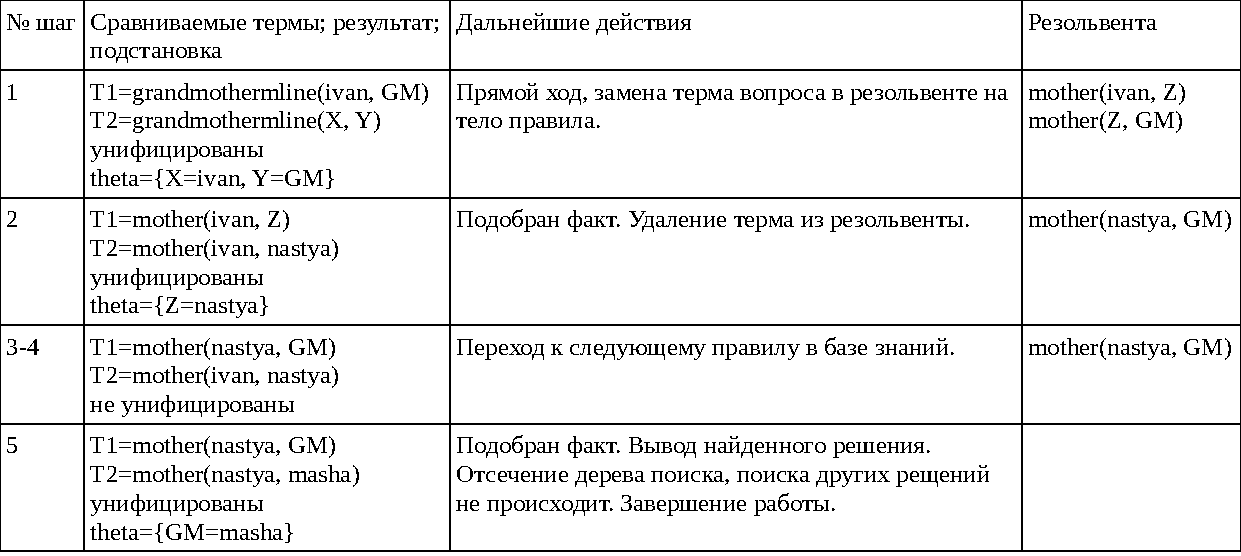
\includegraphics[width=0.95\linewidth]{table.pdf}
\end{center}
